\documentclass[12pt, a4paper]{article}
\usepackage[utf8]{inputenc}
\usepackage{amsmath}
\usepackage{amsfonts}
\usepackage{amsthm}
\usepackage{graphicx}
\usepackage{parskip}
\usepackage{hyperref}
\usepackage{fancyhdr}
\usepackage{lastpage}
\usepackage{tikz}
\usepackage{float}
\usepackage{listings}
\usepackage{color}
\usepackage{caption}
\usepackage[acronym]{glossaries}
\usepackage[nottoc]{tocbibind}
\usepackage[cache=false]{minted}
\usemintedstyle{default}
\newminted{haskell}{frame=lines,framerule=2pt}
\graphicspath{{./images/}}

\tikzstyle{bag} = [align=center]

\lstset{frame=tb,
  language=Haskell,
  aboveskip=3mm,
  belowskip=3mm,
  showstringspaces=false,
  columns=flexible,
  basicstyle={\small\ttfamily},
  numbers=left,
  numberstyle=\tiny\color{gray},
  keywordstyle=\color{blue},
  commentstyle=\color{dkgreen},
  stringstyle=\color{mauve},
  breaklines=true,
  breakatwhitespace=true,
  tabsize=2,
  stepnumber=1,
  escapechar=`
}

\definecolor{dkgreen}{rgb}{0,0.6,0}
\definecolor{gray}{rgb}{0.5,0.5,0.5}
\definecolor{mauve}{rgb}{0.58,0,0.82}

\title{%
      Homework 2 \\
      Experimental Prove of Cukoo Hashing features
}
\author{%
  Juan Pablo Royo Sales \\
  \small{Universitat Politècnica de Catalunya}
}
\date\today

\pagestyle{fancy}
\fancyhf{}
\fancyhead[C]{}
\fancyhead[R]{Juan Pablo Royo Sales - UPC MIRI}
\fancyhead[L]{ADS - Homework 2}
\fancyfoot[L,C]{}
\fancyfoot[R]{Page \thepage{} of \pageref{LastPage}}
\setlength{\headheight}{15pt}
\renewcommand{\headrulewidth}{0.4pt}
\renewcommand{\footrulewidth}{0.4pt}

\makeglossaries

\newacronym{cuk}{CUKOO}{Cukoo Hashing}
\newacronym{ccc}{CCC}{Complex Connected Component}
\newacronym{bpgraph}{BGRAPH}{Bipartite Graph}
\newacronym{haskell}{Haskell}{Haskell Programming Language}

\begin{document}

\maketitle

\section{Introduction}
In this homework I am going to show through experimentation analysis two of the most important features of \acrfull{cuk} that are describe in detail here \cite{cukoo}:

\begin{itemize}
  \item Insertion amortized expected $\theta(1)$
  \item The probability that \acrshort{cuk} contains \acrfull{ccc} in terms of the Hastables that forms a \acrfull{bpgraph} when $m = (1+\epsilon)n$ is $m =O(1/n)$ \cite{kutze}
\end{itemize}

I am going to show through experimental analysis, that empirically we can implement a \acrshort{cuk} that fulfill these properties.

In order to see how the code and resources are organized and where to find all the material need, please check~\ref{appendix} section.

\section{Implementation}
The \acrshort{cuk} implementation that has been done for running this experiments is in \acrfull{haskell}.

I have implemented a full feature \acrshort{cuk} with some limitations:

\begin{haskellcode*}{}
module Data.Hash.Cukoo
  ( create
  , insert
  , delete
  , lookup
  , toList
  , elements
  , rehashed
  , rehashesCount
  , length
  ) where
\end{haskellcode*}

\subsection{Limitations and Assumptions}
The first limitation that is important to pointed out is the \mintinline{haskell}{create} function which creates a new \acrshort{cuk} empty data structure. My implementation does not support multiple Hashtables indirections, and I have worked with a \acrshort{cuk} implementation of \textbf{2} Hashtables.

Another important limitation is that I only allow \mintinline{haskell}{Integer} Positive values $x | x \in \mathbb{N}$. This restriction is allowing me to used \textbf{Unboxed Values} which increase the performance of my Data Type in big order of magnitude. You can check \textbf{Unboxed Values} explanation on \acrshort{haskell} here \cite{unboxed}.

The last limitation or assumption on hour implementation is the viability to work with \textbf{Universal Hash Functions}. Since we know although theoretical is possible, in the real implementations is very hard to achieve, in my implementation I am not working with \textbf{Universal Hash Function} but I am using 2 hash function that use a \textbf{next Prime} of the table expected size and the module of that.

\subsection{Function Interface}
As we can see in the \textbf{export} module list of the \acrshort{cuk} implementation we have the following functions exported and implemented:

\begin{itemize}
  \item Complete \mintinline{haskell}{insert}, \mintinline{haskell}{delete} and \mintinline{haskell}{lookup} functions
  \item \mintinline{haskell}{toList} to convert the \acrshort{cuk} Data Type to a regular list with all the keys in the Hashtable.
  \item \mintinline{haskell}{elements} Count the number of elements in the Hashtable
  \item \mintinline{haskell}{rehashed} Return \mintinline{haskell}{True} if the hash was rehashed on the last \mintinline{haskell}{insert}
  \item \mintinline{rehashesCount} Return the number of rehashes so far.
  \item \mintinline{haskell}{length} Return the length of both internal Hashtables. In fact this is going to return $2M$ where $M$ is the size of 1 of the internal hashtable.
\end{itemize}

\section{Experiments}
In this section I am going to describe what is the setup of the experiment I have prepared and run and what assumptions I am doing.

\subsection{Insert without Rehashing - Average time}\label{sec:ins}
In order to calculate the average time of insertion without rehashing, I am measuring the time of the successful inserts, and only those that after insert the \mintinline{haskell}{rehashed} function returns \mintinline{haskell}{False}.

\begin{listing}[H]
\begin{haskellcode*}{}
insertWithoutRehash' :: Int -> IO [Integer]
insertWithoutRehash' n = do
  idx <- getPositive <$> generate (arbitrary @(Positive Int))
  list <- generate $ shuffle [idx `.`. idx + n]
  let (test, train) = splitAt (n '`div'` 2) list
  fmap catMaybes <$> return $
    runST $ do
      hash <- create
      mapM_ (C.insert hash) $ test
      forM train $ \e -> do
        start <- toNano <$> return (unsafePerformIO getCurrentTime)
        _ <- C.insert hash e
        rehash <- C.rehashed hash
        end <- toNano <$> return (unsafePerformIO getCurrentTime)
        return $ unsafePerformIO $ print start
        let diff = (end - start)
        return $
          if rehash
            then Nothing
            else Just diff
\end{haskellcode*}
\caption{Insert without Rehashing Function}
\label{lst:insertWithoutRehash}
\end{listing}

In the case of this experiment I am running $3000$ iterations of Random lists which size is between $100$ and $10000$ elements.

\subsection{Average Number of Rehashes}\label{sec:rehash}
The other experiment that I have run is the average number of rehashes. In this case what I have done is to run $1000$ iterations, creating Hashtables in each iteration of Random number of elements always greater than $1000$ elements but less than $10000$. In this case, after each creation of the whole iteration I have used \mintinline{haskell}{rehashesCount} function to gather the number of rehashes done and compare with the size of the internal Hashtable which is always going to be $2M$ as i have mentioned in the previous section.

\begin{listing}[H]
\begin{haskellcode*}{}
avgRehashes' :: Int -> IO (Int, Int)
avgRehashes' n = do
  idx <- getPositive <$> generate (arbitrary @(Positive Int))
  list <- generate $ shuffle [idx `.`. idx + n]
  return $
    runST $ do
      hash <- create
      mapM_ (C.insert hash) list
      rehashes <- C.rehashesCount hash
      l        <- C.length hash
      return (l, rehashes)
\end{haskellcode*}
\caption{Rehash Count Experiment Function}
\label{lst:avgRehashes}
\end{listing}

\section{Results}
\subsection{Average Time Insert without Rehash}
After running the experiment described in~\ref{sec:ins} we can draw the following graph with the gathered data.

  \begin{minipage}[t]{\linewidth}
    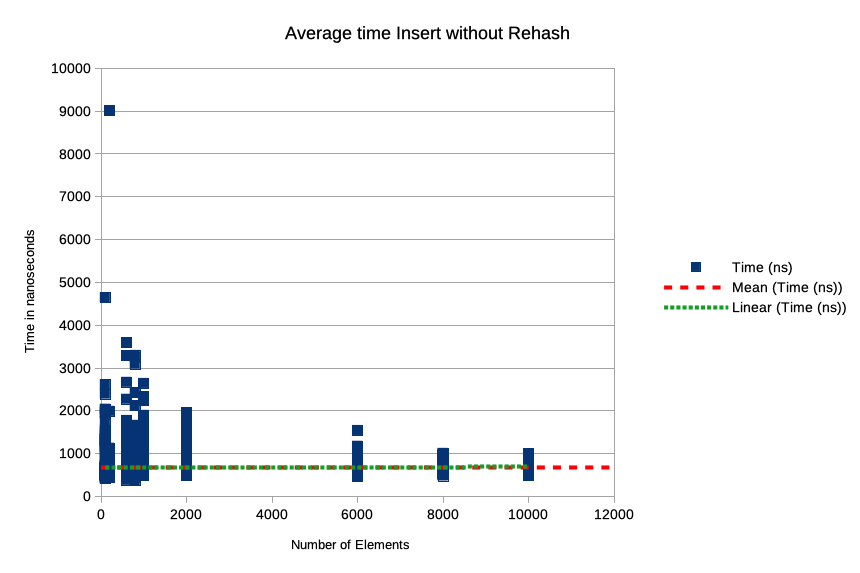
\includegraphics[width=\textwidth]{insert_without_rehash}
    \captionof{figure}{Insert without Rehash Average Time}
    \label{fig:ins_rehash}
  \end{minipage}

  In this graph we can appreciate that no matter the \textbf{Number of Elements} that we insert in the table the average time is mainly in the
  \textit{850 nanoseconds}.

  On the other hand we can appreciate that there are some data points which are far away from the average time, but it is not the majority since the samples are big this is not representative.

  Analyzing the data I have appreciate that those points that are far away from from the \textbf{Mean} are those when the number of elements are small and in consequence when the size of the Hashtable is small too.

  If we take the theoretical \textbf{amortized insert} cost that we state in the Introduction, we can see \textit{w.l.g.} that the time is more or less constant in practice for the majority of the samples.


\subsection{Average Number of Rehashes}
After running the experiments described in~\ref{sec:rehash} we can see the following graph built with the gathered data.


\begin{minipage}[t]{\linewidth}
  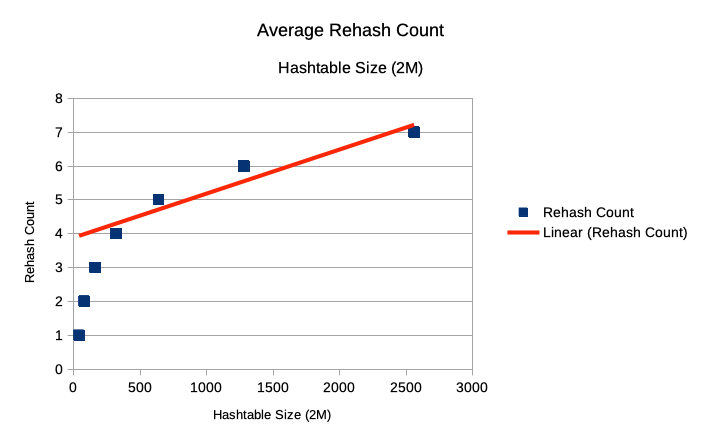
\includegraphics[width=\textwidth]{average_rehash_count_2m}
  \captionof{figure}{Average Rehash Count vs. Hashtable Size}
  \label{fig:rehash_avg_2m}
\end{minipage}


The first analysis we can state is comparing the number of \textbf{rehashes} with respect to the size of Hashtables.

As we can appreciate from the results the total number of rehashes is never above $7$ and never grows abruptly in spite the number of elements of being inserted is increasing faster with the number of iterations. We are going to see that in a more clear way in the following plot.

\begin{minipage}[t]{\linewidth}
  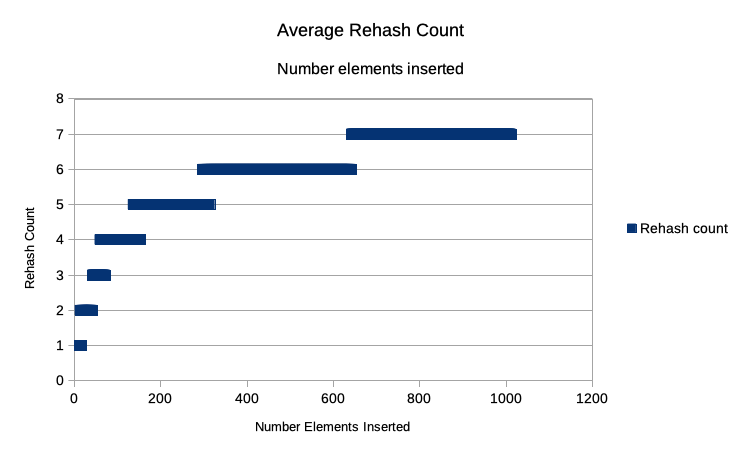
\includegraphics[width=\textwidth]{average_rehash_count_n}
  \captionof{figure}{Average Rehash Count vs. Number Elements}
  \label{fig:rehash_avg_n}
\end{minipage}

In this graphic we can clearly see that in spite the number of elements grows and even double as the iterations take place, we never go above $7$. This is a great approximation to the probability state in the introduction that says that in this \acrshort{bpgraph} is $O(1/n)$.

\section{Conclusion}
In conclusion I can state that this structure is very close to its theoretical statement.

On the one hand I feel more confident with the empirical results of \textbf{rehash count} rather than \textbf{average time on insertion}.

One of the possibility to have many data points far away the average in the case of Insertion is the real viability to work with \textbf{Universal Hash Function} which implies that I am having to much collisions and unsuccessful inserts which lead me to a worst time in some cases for insertions. Because of that for big number since the Hashtables are larger i am getting less collisions and more successful inserts, therefore less insertion average time.


\appendix\label{appendix}
\section{Haskell Code}
\subsection{Source Code}
In the source code there are 2 folders with code:

\begin{itemize}
  \item \textbf{app}: \mintinline{haskell}{Main.hs} which contains the main entry point of the program that run all the experiment
  \item \textbf{src}: \mintinline{haskell}{Experiments.hs} contains the experiments and \mintinline{haskell}{Data/Hash/Cukoo.hs} that contains the implementation of \acrshort{cuk}
\end{itemize}

\subsection{Run the Code}
All the solution has been coded with \textbf{Stack} \cite{stack} version 2.1.3 or higher. It is a prerequisite to install \textit{stack} for running this code.

\subsubsection{Running Experiments}

In order to run the experiments just do the following:

\begin{lstlisting}[language=Haskell,title={Running Experiments}]
shell> stack build
shell> stack exec cukoo
\end{lstlisting}

\section{Generated Reports}
All the Generated Reports that has been used to build this document are under \mintinline{haskell}{output} folder.


\section{Report PDF Document}
This report document is under \mintinline{haskell}{doc} folder alongside images that are embedded in this report.


\bibliographystyle{alpha}
\bibliography{report}

\printglossary[type=\acronymtype]

\end{document}

